\documentclass[conference]{IEEEtran}
\IEEEoverridecommandlockouts
% The preceding line is only needed to identify funding in the first footnote. If that is unneeded, please comment it out.
\usepackage{cite}
\usepackage{amsmath,amssymb,amsfonts}
\usepackage{algorithmic}
\usepackage{graphicx}
\usepackage{textcomp}
\usepackage{xcolor}
\usepackage{float}
\def\BibTeX{{\rm B\kern-.05em{\sc i\kern-.025em b}\kern-.08em
    T\kern-.1667em\lower.7ex\hbox{E}\kern-.125emX}}
\begin{document}

\title{CENG466, Fall 2022, THE 3\\

}

\author{\IEEEauthorblockN{1\textsuperscript{st} Fırat Ağış}
\IEEEauthorblockA{\textit{Department of Computer Engineering} \\
\textit{Middle East Technical University}\\
Ankara, Turkey \\
e2236867@ceng.metu.edu.tr}
\and
\IEEEauthorblockN{2\textsuperscript{nd} Robin Koç}
\IEEEauthorblockA{\textit{Department of Computer Engineering} \\
\textit{Middle East Technical University}\\
Ankara, Turkey \\
e2468718@ceng.metu.edu.tr}
}

\maketitle

\begin{abstract}

\end{abstract}

\begin{IEEEkeywords}

\end{IEEEkeywords}

\section{Face Detection}
For face detection, we propose an algorithm that use k-means to separate color groups, chooses the color group that is most likely to include skin colors and then uses morphological operations and convolution operation to detect areas that are most likely to include faces in the image. Our algorithm posses 3 distinct stages:
\begin{enumerate}
	\item \textit{Preprocessing:} Process the image to be more suitable for our algorithm and performs some processes to make the algorithm run a lot faster.
	\item \textit{K-Means:} Using k-means algorithm with randomized starting means to detect the pixels that are most likely to be in the color of skin tones.
	\item \textit{Context Based Postprocessing:} Using morphological operations and convolution operation to detect which clusters of the pixels that are found in the previous step to be the part of a face.
\end{enumerate}
\subsection{Preprocessing}
\begin{enumerate}
	\item \label{step:A1} We first read the relevant image. Shown in Row 1 of Figure \ref{fig:pro1}.
	\item \label{step:A2} (Optional) We perform histogram equalization to differentiate skin tones from similar colors in the image, most notably, the leaves in the 1\_source.png and shirt and hair in 3\_sources.png. Shown in Row 2 of Figure \ref{fig:pro1}.
	\item \label{step:A3} (Optional) We down-sampled the 2\_source.png by a factor of 9 in order to complete the algorithm in a reasonable time. 
	\item \label{step:A4} We bit-sliced all images, eliminating the least significant bit. Colors that are differentiated by a single bit are most likely to be in the same color group, meaning this operation affected the quality of the k-means algorithm minimally while reducing the size of the color space by a factor of $2^3=8$. Shown in Row 3 of Figure \ref{fig:pro1}.
\end{enumerate}
\subsection{K-Means}
\begin{figure}[h]
    \centering
    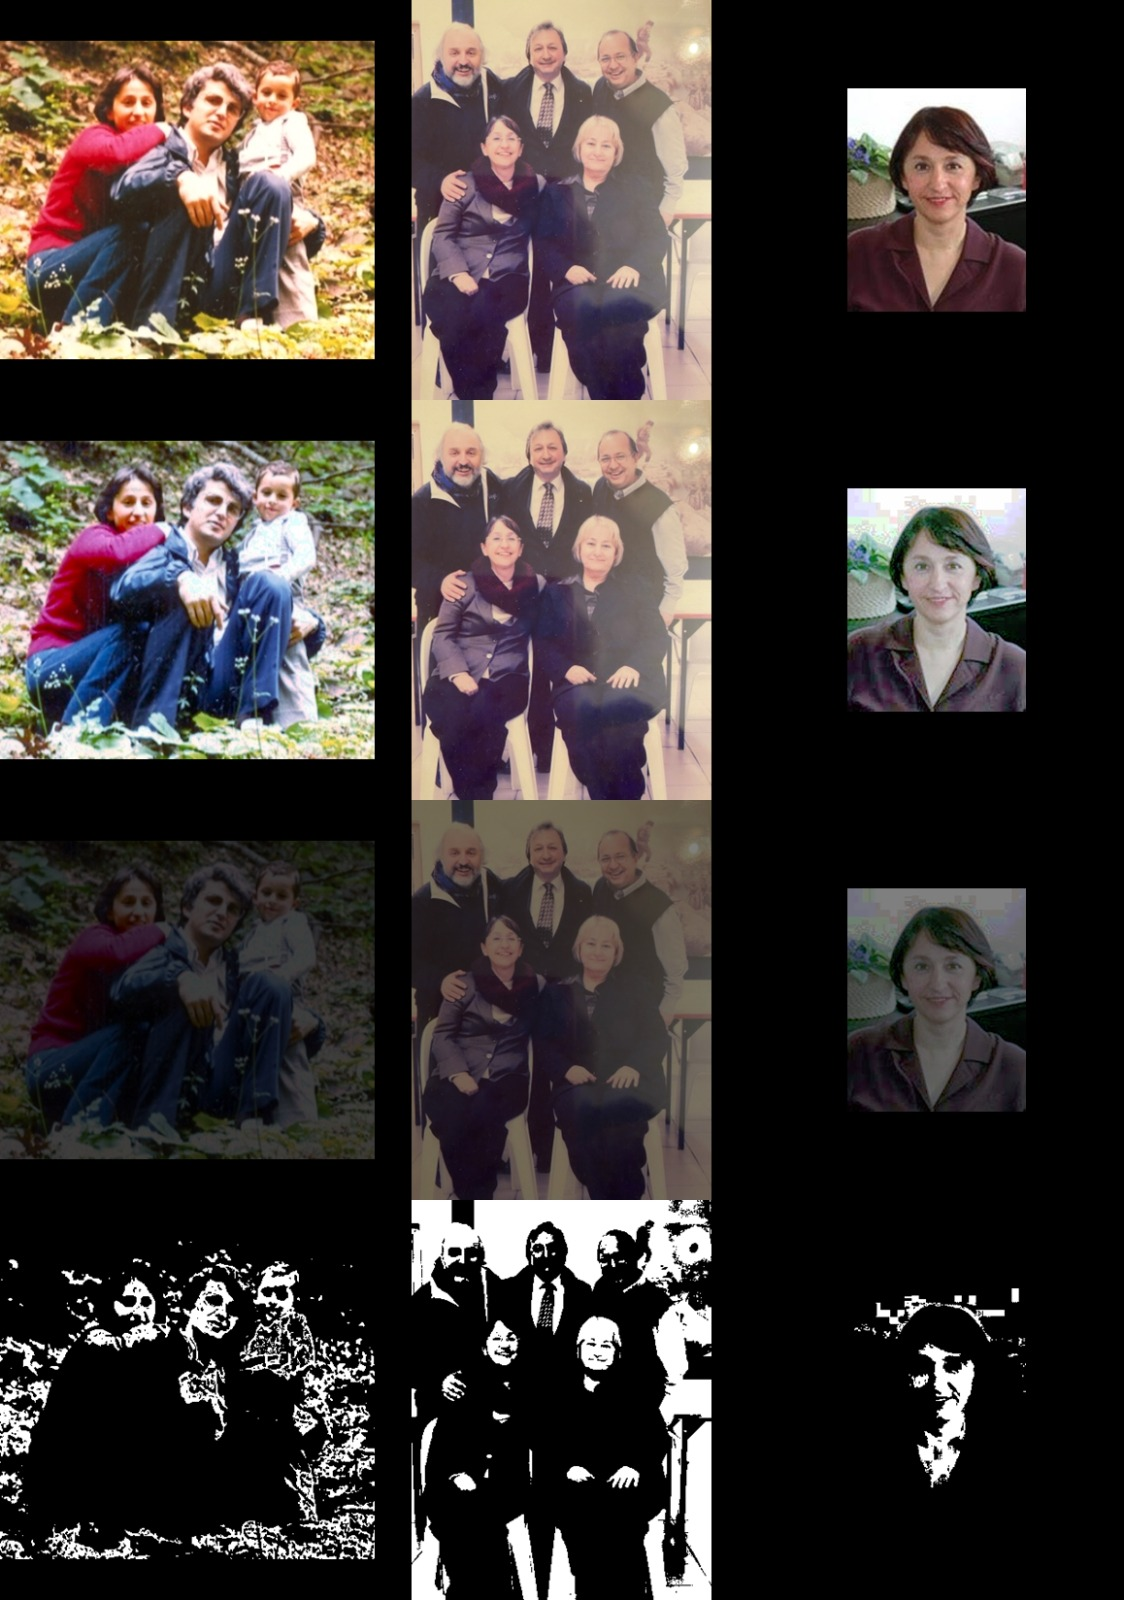
\includegraphics[width=0.4\textwidth]{resources/Progress 1.jpeg}
    \caption{Face detection progress for preprocessing and k-means stages}
    \label{fig:pro1}
\end{figure}
\begin{enumerate}
	\item \label{step:B1} We performed k-means algorithm with randomized initial means, acquiring means and colors closest to that means.
	\item \label{step:B2} We only took the colors whose means have the greatest red component using the knowledge that all faces are reddish in the context of color space.
	\item \label{step:B3} We eliminated any colors whose red component is less then their blue or green component using the same logic as the previous step. Shown in Row 4 of Figure \ref{fig:pro1}.
\end{enumerate}

\subsection{Context Based Postprocessing}
\begin{figure}[h]
    \centering
    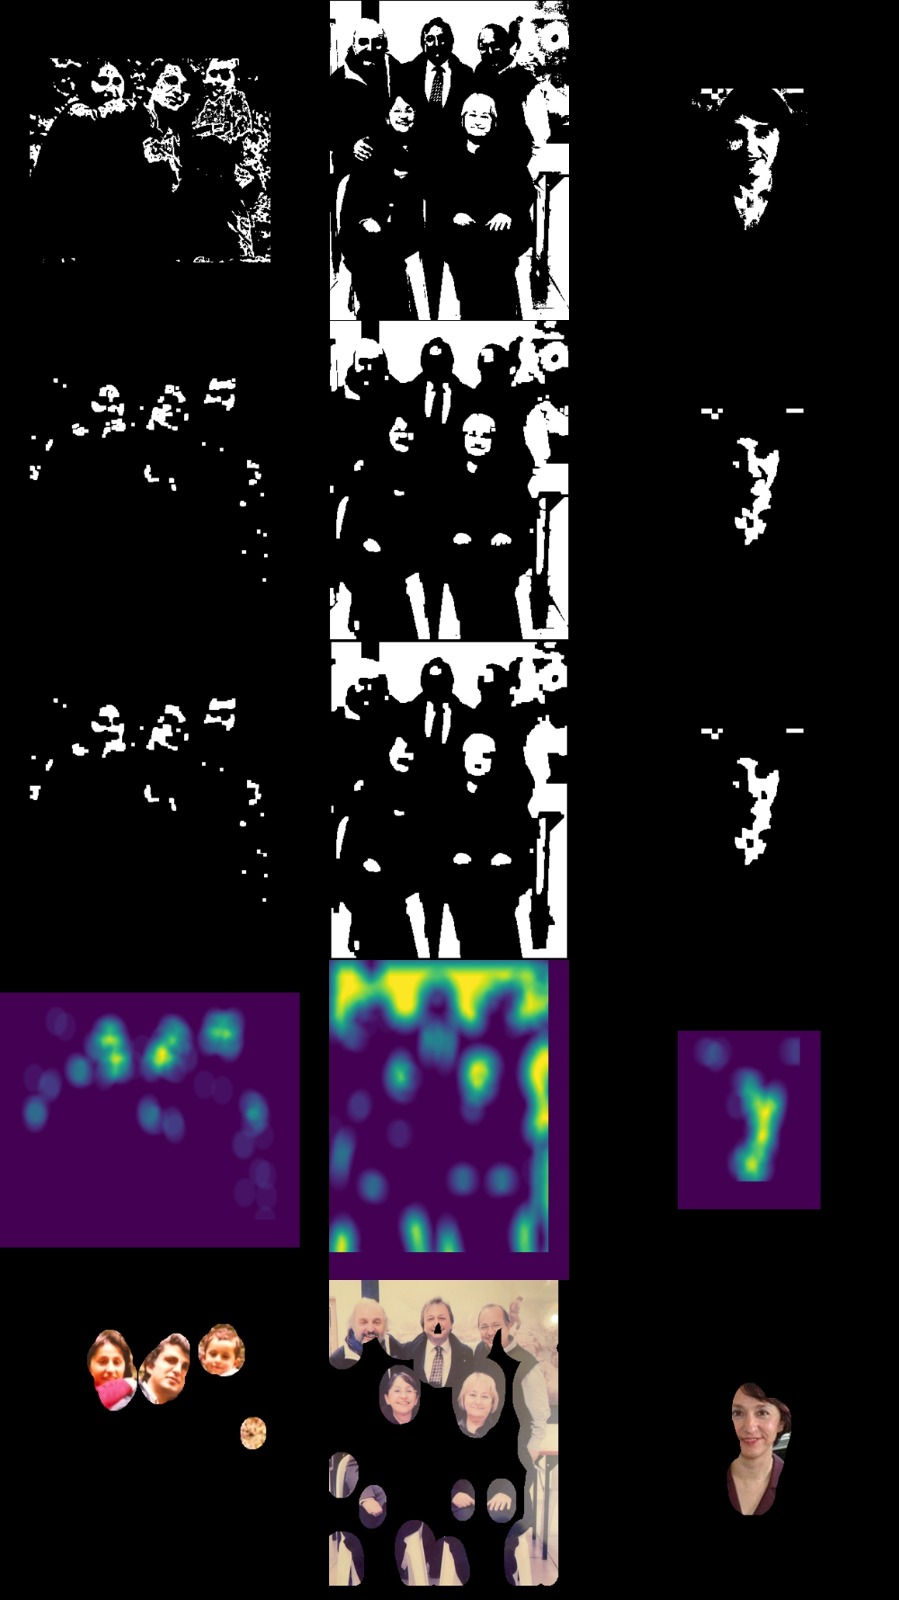
\includegraphics[width=0.4\textwidth]{resources/Progress 2.jpeg}
    \caption{Face detection progress for postprocessing stage}
    \label{fig:pro2}
\end{figure}
\begin{enumerate}
	\item \label{step:C1} (Optional) While processing 1\_source.png and 3\_sources.png, we used the assumption of faces being the central focus of images to eliminate pixels on the outer parts of the image. Shown in Row 1 of Figure \ref{fig:pro2}.
	\item \label{step:C2} We used opening operation with a 5x5 element to eliminate noise from the image. Shown in Row 2 of Figure \ref{fig:pro2}.
	\item \label{step:C3} We used closing operation with a 5x5 element to fix regions that are broken up during the previous step. Shown in Row 3 of Figure \ref{fig:pro2}.
	\item \label{step:C4} We used convolution with a elliptical mask, mimicking the shape of he face to determine locations where a face may lie. Shown in Row 4 of Figure \ref{fig:pro2}.
	\item \label{step:C5} We used thresholding to the result of the convolution, including the parts of the image that passed the tresholding, concluding the algorithm. Shown in Row 5 of Figure \ref{fig:pro2}.
\end{enumerate}
\subsection{Design Process}
After the implementation of basic k-means algorithm, execution time of the algorithm limited the speed of our further progress by trying different processes. For that reason, we implemented the preprocessing steps \ref{step:A3} and \ref{step:A4}.

Then we looked at commonalities between regions that make up the face, which brought us the reasoning we used in the k-means steps \ref{step:B2} and \ref{step:B3}.

After that, we experimented with histogram equalization to differentiate colors easier.

When we arrived at the final result of k-means, given in Row 4 of Figure \ref{fig:pro1}, we determined the noise created by similarly colored regions to be a problem. To solve it, we implemented opening and closing mentioned in the postprocessing steps \ref{step:C2} and \ref{step:C3}. For the noise not eliminated by these steps, around the edge of the image for 1\_source.png, we implemented the postprocessing step \ref{step:C1}.

Morphological operations didn't eliminated all non-face regions. To distinguish regions that are face shaped from others, we finally implemented the postprocessing steps \ref{step:C4} and \ref{step:C5}.
\subsection{Results}
\begin{figure}[h]
    \centering
    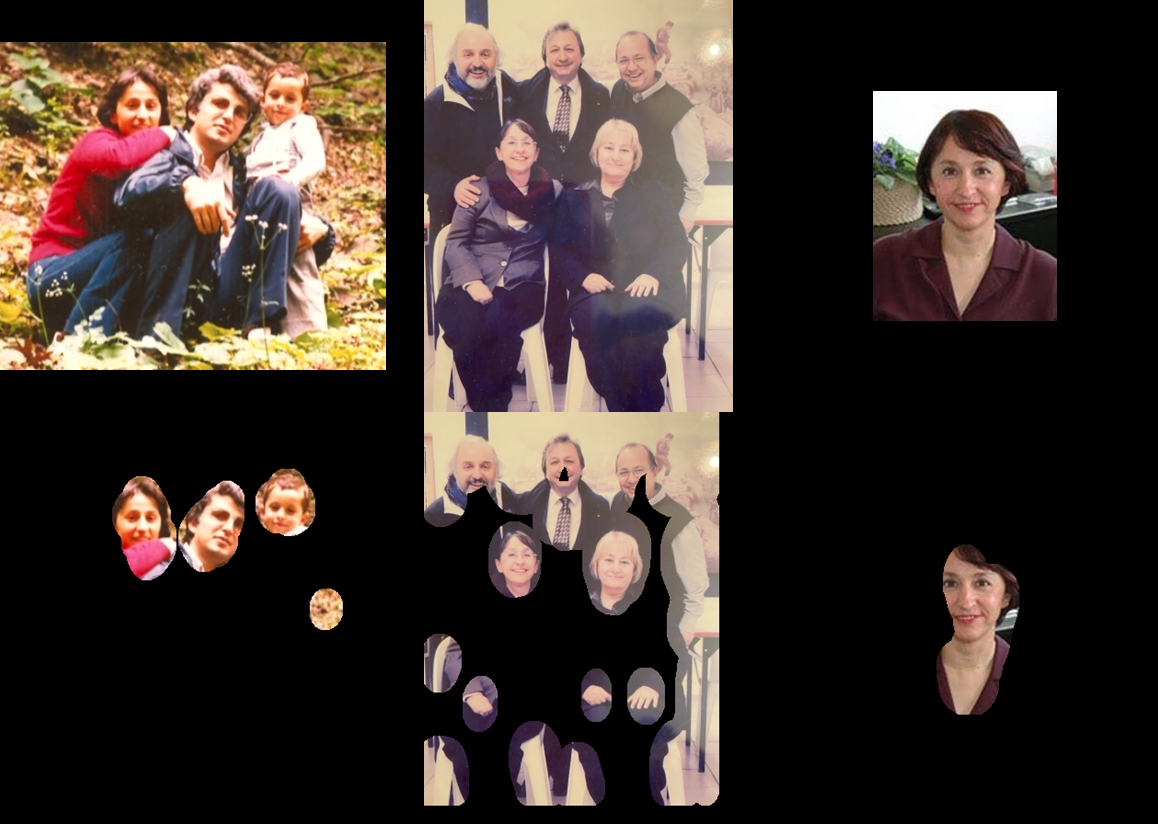
\includegraphics[width=0.4\textwidth]{resources/End Result Compare.jpeg}
    \caption{Original images and the end products}
    \label{fig:end}
\end{figure}
When we looked at the output of the algorithm, given in Figure \ref{fig:end}, we can clearly see that it is quite accurate at finding locations that contains skin colors, while as seen in 2\_faces.png, when the color space is limited, like the yellow saturation of the image, while it eliminates many non-face areas, color and even the shape information is not sufficient to perfectly detect only faces. But when dealing with more non-extreme example, such as 1\_source.png and 3\_source.png, false positives are very limited and all faces are detected. We can thank the postprocessing stage for eliminating false positives while keeping the faces, as a less violent method would create even more false positives and a more violent method would not guarantee the detection of all faces.
\section{Pseudo-coloring}
\subsection{Coloring Grayscale Images}
In a grayscale image we have 256 discrete values for every pixel that represent how much black or how much white the pixel is. 0 being black pixel and 256 being white pixel. In a multichannel image we have values ranging from 0 to 256 for every channel which are red, green and blue for rgb images. Now what we need is a function or set that maps gray values in given grayscale images to rgb values in the given source images. We know that our map should be one to one and need to take values between 0 and 256 and should give a 3 number ranging between 0 to 256 that represents the red green and blue values. For this we had couple of steps:
\begin{enumerate}
    \item Creating a palette
    \item Processing the palette
    \item Mapping the grayscale image
\end{enumerate}

To create a map for grayscale values to rgb values we need to first find corresponding gray values for each rgb value trio. We can use different equations for this, we can take the average of the channels, we can take minimum or maximum of the channels, we can take weighted averages etc. The goal is to create a single value between 0 and 256 from three values that are rgb. We thought logical way for this would be using the luminance. Normally when we look at an image we will probably say that the darker colors must be represented by darker gray values and lighter one by the lighter gray values but since the human visual system does not correspond to the rgb color system we can not just say bigger rgb values would be lighter. Closest to human visual system would be using the luminance, to compute luminance we can take the weighted average of the rgb values with the weights (0.2989, 0.5870, 0.1140). This values are used in many systems for computing the luminance. 

\begin{figure}[H]
    \centering
    
\includegraphics[width=0.4\textwidth]{resources/4_source.png}
    \caption{Source image to use rgb values from}
    \label{fig:image_4_source}
\end{figure}

\begin{figure}[H]
    \centering
    
\includegraphics[width=0.4\textwidth]{resources/4.png}
    \caption{We can guess that the lightest value would represent the color yellow in the picture}
    \label{fig:image_4_gray}
\end{figure}


\subsection{Extracting Palette from RGB Image}
To extract a palette we created an empty palette with 0 value then we computed the luminance values from red green and blue values of source image and used them as indexes. Luminance values would represent the index of the palette and the palette would hold the rgb value the index created from like, palette[luminance] = (red, green, blue). This gave us a rather empty looking palette. 

\begin{figure}[H]
    \centering
    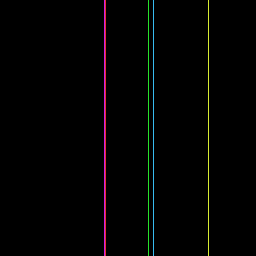
\includegraphics[width=0.4\textwidth]{resources/4_palette.png}
    \caption{Unprocessed palette}
    \label{fig:image_4_palette}
\end{figure}

\subsection{Processing the Palette}
Now the gray values from the image may not correspond to the non-zero luminance values from the palette for this we thought of filling zeros of the palette with the weighted average of the two closest non-zero values of it using spatial distances. The result was continuous looking palette with every grayscale value corresponding to a rgb value where black values were still black and white values were still white.

\begin{figure}[H]
    \centering
    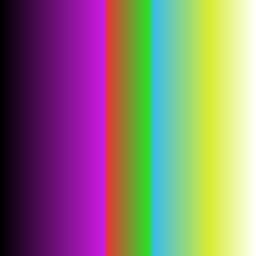
\includegraphics[width=0.4\textwidth]{resources/4_filled_palette.png}
    \caption{Filled palette}
    \label{fig:image_4_filled_palette}
\end{figure}

\subsection{Using Palette to Color Grayscale Images}
Now the easy part was using the grayscale values as indexes of palette and mapping those rgb values to the image for coloring like, colored\_image = palette[gray\_scale\_images\_values]. Results was really good for some images and good enough for some others.

\begin{figure}[H]
    \centering
    
\includegraphics[width=0.4\textwidth]{resources/4_colored.png}
    \caption{Colored version of image 4}
    \label{fig:image_4_colored}
\end{figure}

\begin{figure}[H]
    \centering
    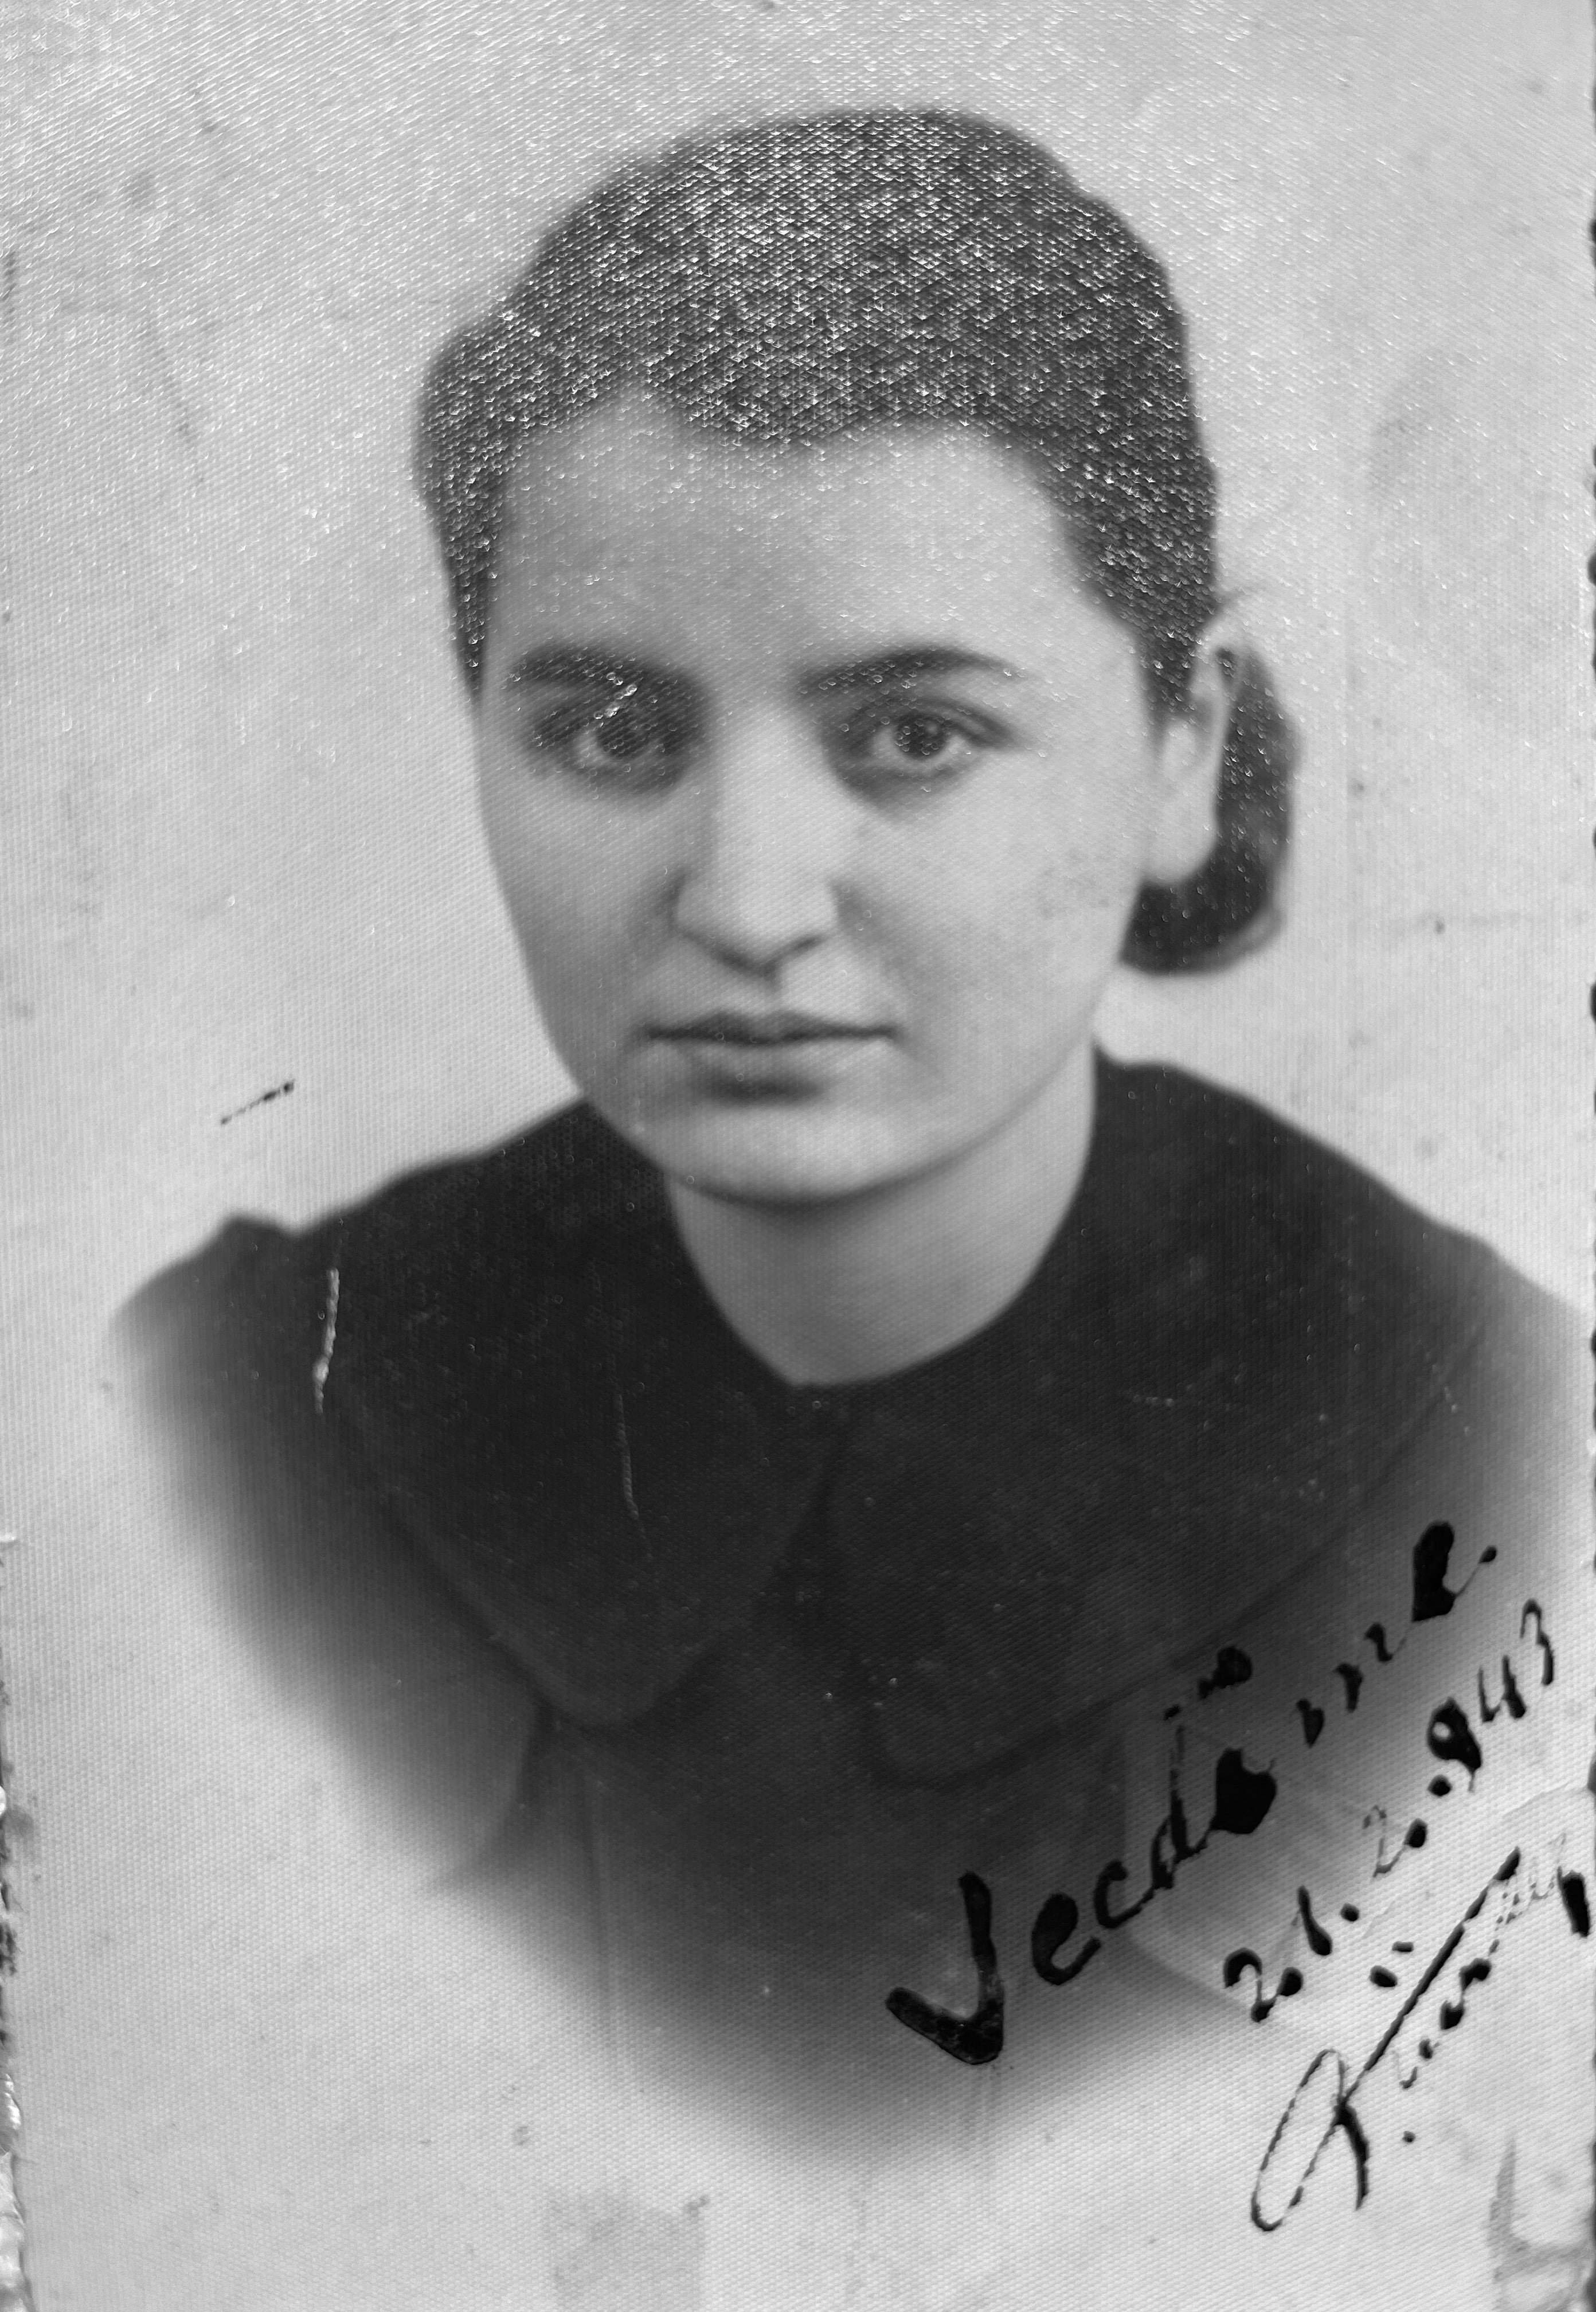
\includegraphics[width=0.4\textwidth]{resources/3.jpg}
    \caption{Grayscale image 3}
    \label{fig:image_4_colored}
\end{figure}

\begin{figure}[H]
    \centering
    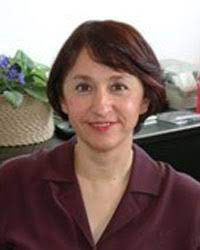
\includegraphics[width=0.4\textwidth]{resources/3_source.png}
    \caption{Source image for image 3}
    \label{fig:image_4_colored}
\end{figure}

\begin{figure}[H]
    \centering
    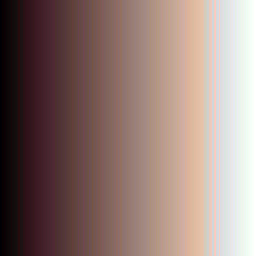
\includegraphics[width=0.4\textwidth]{resources/3_filled_palette.png}
    \caption{Processed palette from source 3}
    \label{fig:image_4_colored}
\end{figure}

\begin{figure}[H]
    \centering
    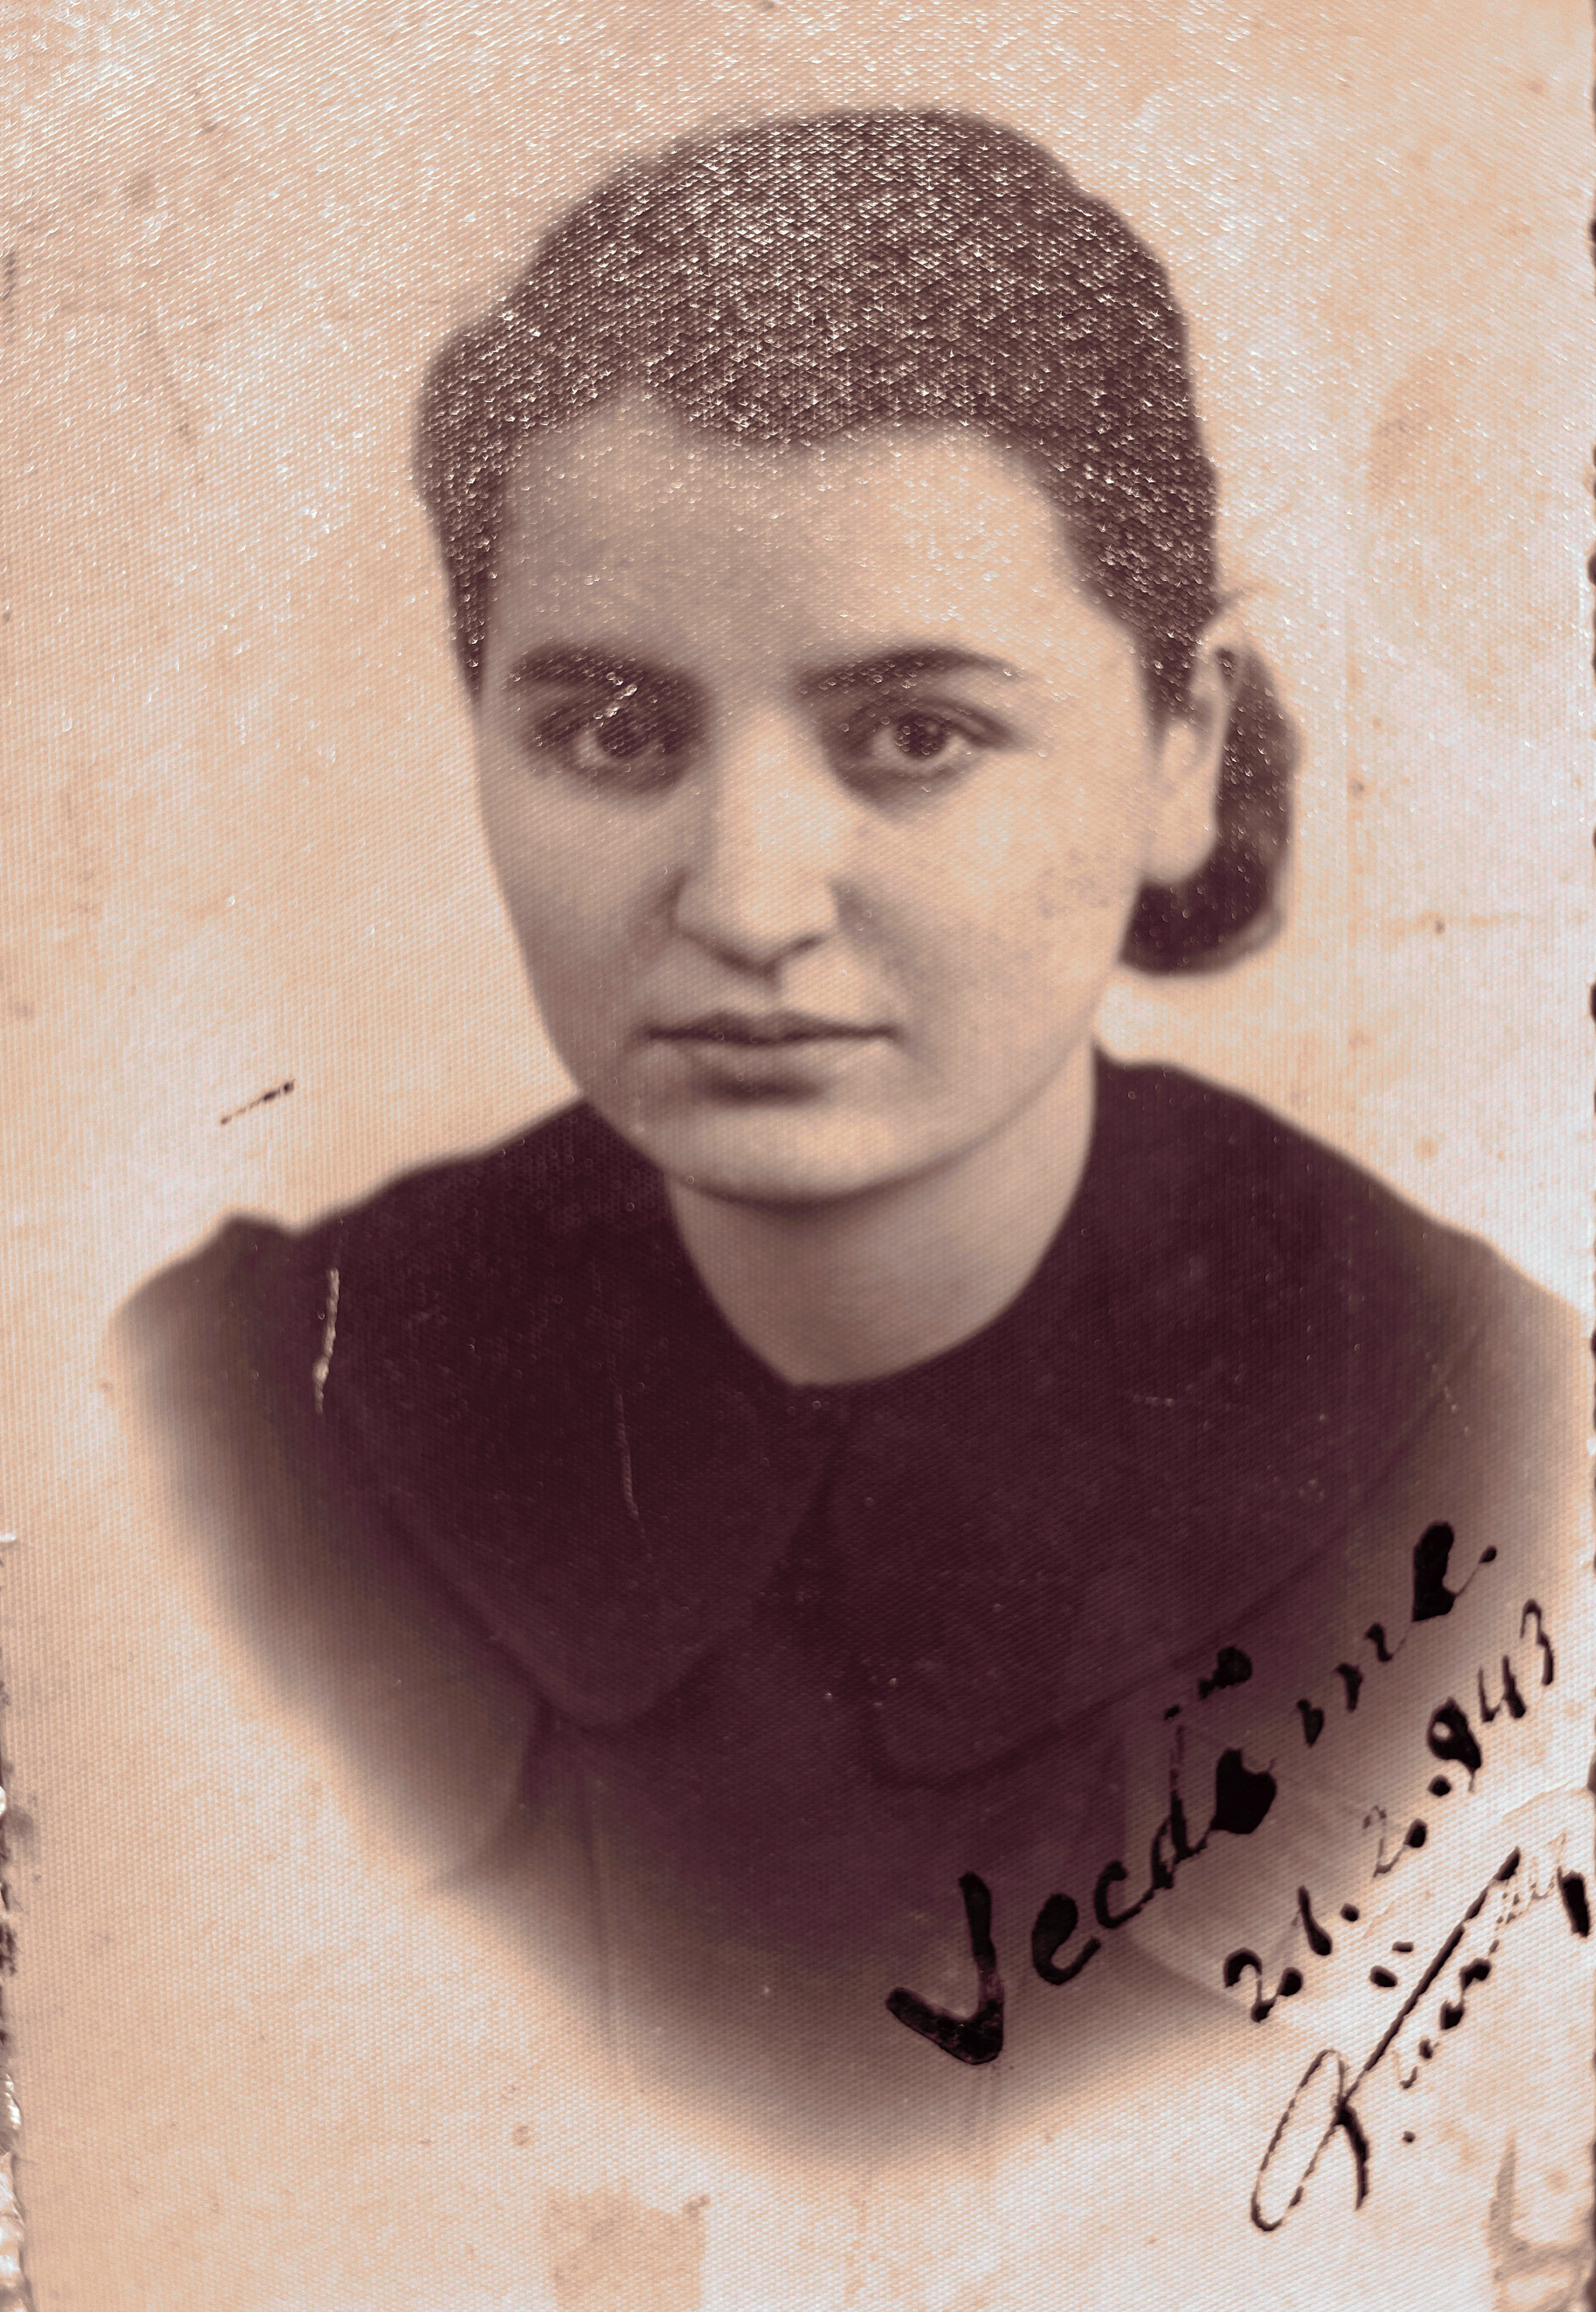
\includegraphics[width=0.4\textwidth]{resources/3_colored.jpg}
    \caption{Colored version of image 3}
    \label{fig:image_4_colored}
\end{figure}

We can see that our coloring algorithm does a bit of averaging but since these are a bit washed out old photos we are colorizing this was an expected result for us.

\subsection{Rgb, Hsi and Histograms}
We have different color systems for different purposes and usage areas, two of them we used in this homework are hsi and rgb. Hsi color space has three components named hue, saturation and intensity. These can be summarized as hue is which color are we using, saturation is  degree of how much gray the color contains (sharper or washed out colors) and intensity is about brightness. We can convert values from these color systems to each other with 3 particular equations. Since these are just representations and we can convert from one of them to the other we do not lose information but they tend to give us advantages over the others in some application areas. For example the hsi color space is modeled after human visual system and easier to associate with how we see the colors. 

We can extract the histograms from a hsi image just as same as rgb one. We have different curves plotted in same histogram for red, green and blue channel in one and same for hue, saturation and intensity in the others. 

\begin{figure}[H]
    \centering
    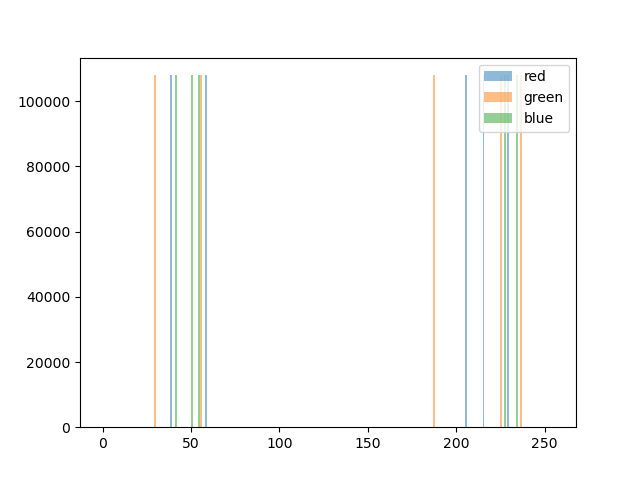
\includegraphics[width=0.4\textwidth]{resources/4_rgb_histogram.png}
    \caption{Rgb histogram of colored image 4}
    \label{fig:image_4_rgb_histogram}
\end{figure}

We can see that there are a lot of 0 values in many of the buckets in histogram, this is due to the low number of color variation in the image 4 (5 different colors i particular). Same thing goes for the hsi histogram.

\begin{figure}[H]
    \centering
    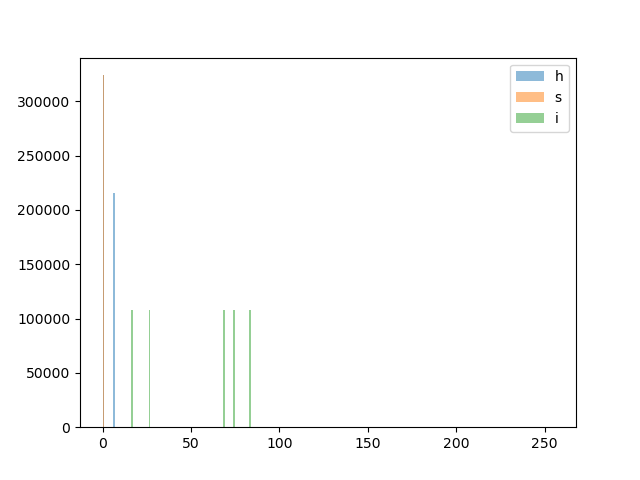
\includegraphics[width=0.4\textwidth]{resources/4_hsi_histogram.png}
    \caption{Hsi histogram of colored image 4}
    \label{fig:image_4_hsi_histogram}
\end{figure}

\begin{figure}[H]
    \centering
    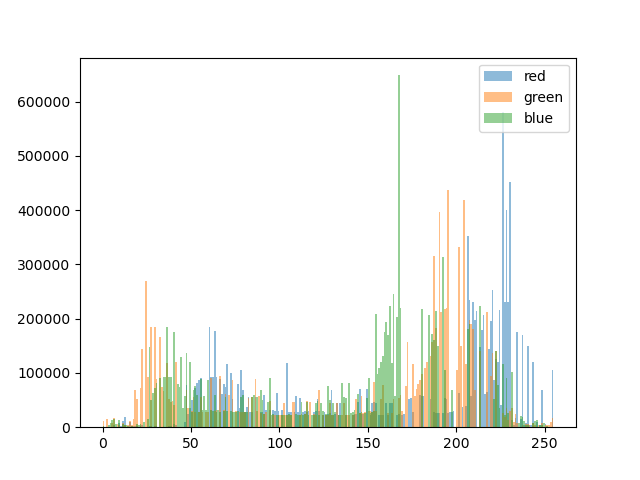
\includegraphics[width=0.4\textwidth]{resources/3_rgb_histogram.png}
    \caption{Rgb histogram of colored image 3}
    \label{fig:image_3_rgb_histogram}
\end{figure}

We can see that the intensity curve is more ranged than the hue and saturation. This is because intensity channel acts as almost a mapping to a grayscale image and contains most of the information in the image. 

\begin{figure}[H]
    \centering
    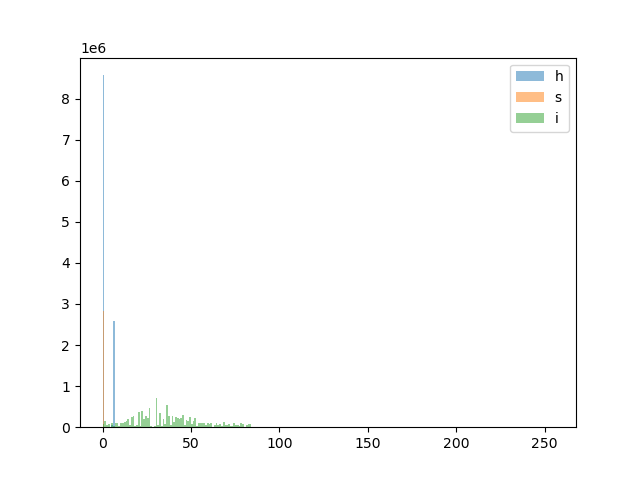
\includegraphics[width=0.4\textwidth]{resources/3_hsi_histogram.png}
    \caption{Hsi histogram of colored image 3}
    \label{fig:image_3_hsi_histogram}
\end{figure}

\subsection{Edge Detection in RGB and HSI}
In this homework we were tasked with detecting edges from the images using gradient filters. For this purpose we used Sobel filters. We have two Sobel filters for horizontal edges and vertical edges named $Sobel_h$  and $Sobel_v$. Convoluting these filters gives us two different edges maps for horizontal and vertical edges. And combining these two will give us all the edges since every edge is made of vertical and horizontal components. We can do this in both rgb and hsi color space. 

$Sobel_h$:  
$\begin{bmatrix}
-1 & 0 & 1\\
-2 & 0 & 2\\
-1 & 0 & 1
\end{bmatrix}$
$Sobel_v$:  
$\begin{bmatrix}
-1 & -2 & -1\\
0 & 0 & 0\\
1 & 2 & 1
\end{bmatrix}$


To do this we can find edges for red, blue and green channels and add them all to get the complete edge map.

\begin{figure}[H]
    \centering
    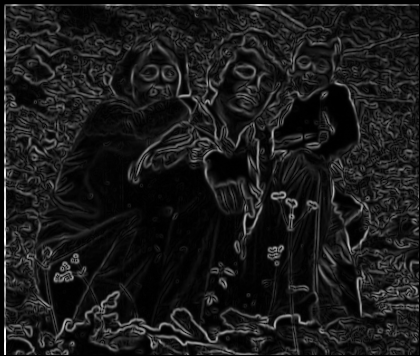
\includegraphics[width=0.4\textwidth]{resources/1_rgb_colored_edges.png}
    \caption{Edge map of image 1 in rgb color space}
    \label{fig:image_1_rgb_edges}
\end{figure}

\begin{figure}[H]
    \centering
    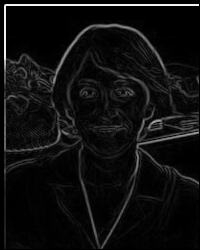
\includegraphics[width=0.4\textwidth]{resources/3_rgb_colored_edges.png}
    \caption{Edge map of image 3 in rgb color space}
    \label{fig:image_3_rgb_edges}
\end{figure}

To do this edge detecting method in hsi color space we almost only need the intensity channel. As we said the intensity channel of the hsi color space contains most of the information in the image. We tried using only the intensity channel for the edge detection and got results identical to the human eye.

\begin{figure}[H]
    \centering
    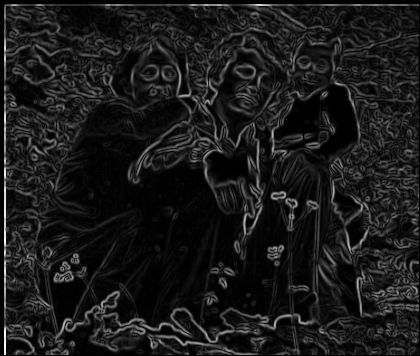
\includegraphics[width=0.4\textwidth]{resources/1_hsi_colored_edges.png}
    \caption{Edge map of image 1 in hsi color space}
    \label{fig:image_1_hsi_edges}
\end{figure}

\begin{figure}[H]
    \centering
    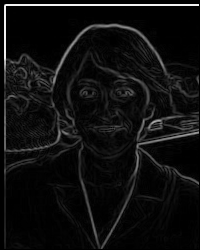
\includegraphics[width=0.4\textwidth]{resources/3_hsi_colored_edges.png}
    \caption{Edge map of image 3 in hsi color space}
    \label{fig:image_3_hsi_edges}
\end{figure}

\section{Dependencies}
We used following libraries for the described reasons.
\begin{itemize}
	\item \textbf{os:} Handling non-existent input or output paths.
	\item \textbf{math:} Performing square root operation.
	\item \textbf{numpy:} Executing array and matrix operations.
	\item \textbf{PIL:} Reading images and converting them to arrays.
	\item \textbf{mathplotlib:} Creating histograms as graphics and writing arrays as image files.
\end{itemize}

\end{document}
